%%%%%%%%%%%%%%%%%%%%%%%%%%%%%%%%%%%%%%%%%%%%%%
\logvartrue
\chapter{Background}
%%%%%%%%%%%%%%%%%%%%%%%%%%%%%%%%%%%%%%%%%%%%%%

Bacteria are often cited as examples of one of the Earth's most primitive living forms. Unfortunately, they are still associated almost exclusively to infection diseases. The reality is rather different, in fact only a very small fraction of bacteria is able to cause infections in contrast to a highly diversified and beneficial bacterial world. Most of them not only reciprocally support each other but their immensely varied and efficient metabolism also defines and sustains balanced environments (the biosphere). Solidarity among bacterial cells is one of their most important characteristic. Even infection-causing bacteria are able to benefit from this solidarity, making them more resilient and ``inventive'' than isolated species. In the last 20 years, the development of genomic tools have revolutionized microbial ecological studies and strongly expanded our view on this previously under appreciated microbial world. It is encouraging to see that evolution and ecology are now emerging as regular subjects within microbiology. The next decade should be one of gradually changing and enlarging perspective regarding the place of bacteriology in the biological sciences. There are now comforting signs that we are moving towards a deeper and more realistic appreciation of the roles played by bacteria on our planet.

\section{The Bacterial world}
Microorganisms are essentially everywhere in nature and they have been integral to the history and function of life on Earth. However, until very recently, their importance has been appreciated by only a few specialist. Indeed, bacteria are still most often considered from an anthropocentric point of view, focusing our attention only on the relatively few pathological species and the potential of microorganisms to provide us with useful products and services (\textbf{da mettere un paio di references}). This is a very constrained perspective if we think that bacteria have been the sole form of life on Earth for some two billion years, playing central roles in climatic, geological, geochemical, and biological evolution \cite{cavalier2006cell}.\\
The bacterial world contains a highly heterogeneous group of organisms sharing only one common characteristic, their small size. The patterns of bacteria distribution are influenced by environmental factors such as temperature, pH, salinity, pressure, the presence of nutrients and the sources of carbon and energy \citep{gerhard1986bacterial}. These factors are able to shape Earth's bacterial communities distribution in respect to both space and time, influencing the selective proliferation of a set of bacteria in a distinct environment, based on their metabolic characteristics. Bacteria can use many different types of metabolic strategies and bacterial species can often be differentiated from each other based on their metabolic characteristics. The specific metabolic properties of a microbe are one of the major factors in determining that microbe’s ecological niche, and they can be used to classify bacteria in different metabolic groups (Figure ~\ref{fig:bacmet}). Thanks to their high variability, bacteria have been, and still are able to colonize almost every ecological niche in nature.\\
\begin{figure}[!tb]
	\centering
	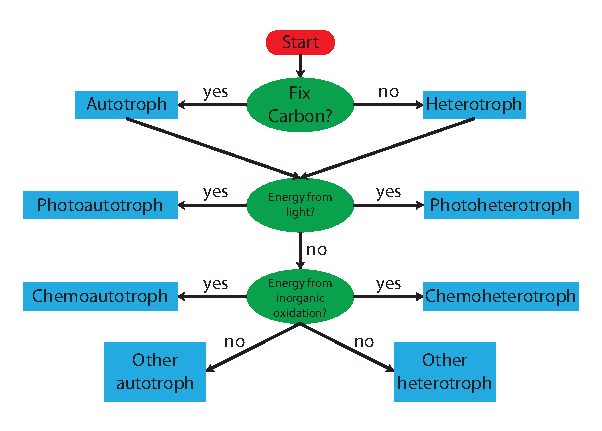
\includegraphics[width=0.7\textwidth]{./figures/Introduction/bacterial_metabolism}
  	\caption{General flowchart used for metabolic classification of bacteria. \label{fig:bacmet}}
\end{figure}
Giving their ability to thrive in a vast set of different environments, bacteria play pivotal roles in several biogeochemical cycles and are responsible for the cycling of organic compounds. They have been found in all kind of environments ranging from the human gut \cite{walter2011human}, to the rhizosphere \cite{philippot2013going}, to conventionally inhospitable habitats such as acid mine run-off \cite{simmons2008population} and geothermal hot springs 	\cite{sharp2014humboldt}. Studies based on cultured microbes have revealed that they are critical components of these environments providing them with essential services \cite{van2008unseen, arrigo2004marine}. For example, the Earth's cycles of hydrogen, carbon, nitrogen, oxygen and sulphur are driven largely by microbial catalysed redox reactions (Figure \ref{}). These reactions require multimeric protein complexes evolved exclusively in microorganism such as bacteria \cite{falkowski2008microbial}. However, a large part of these processes is still unknown making the study of bacterial functions indispensable for the complete comprehension of the dynamics able to modify our planet.\\





%%-----------
%% Backmatter
%%-----------
\backmatter
\chaptermark{Bibliography}
\renewcommand{\sectionmark}[1]{\markright{#1}}
\bibliographystyle{unsrt}                           %Use alpha codes for references
\sectionmark{Bibliography}
\addcontentsline{toc}{chapter}{Bibliography}        %Force addition of Bibliography to TOC    
\bibliography{References}